

\documentclass{article}

\usepackage[utf8]{inputenc}

\usepackage{amsmath, bm}
\usepackage{graphicx}
\usepackage{amssymb}
\usepackage{float}
\usepackage{caption}
\usepackage{subcaption}
\usepackage{hyperref}
\usepackage{tikz}
\usepackage{layout}

\usepackage[margin=1in]{geometry}
\usepackage{listings}
\usepackage{xcolor}
\usepackage{color, colortbl}
\usepackage{textgreek}
\usepackage{mathrsfs}
\usepackage{booktabs}

\usepackage{titlesec}

\titleformat{\subsubsection}
  {\normalfont\selectfont}{\thesubsubsection}{1em}{}

\usetikzlibrary{calc}
\usetikzlibrary{angles,quotes} % for pic
\usetikzlibrary{patterns,snakes}
\usetikzlibrary{arrows}
\tikzset{>=latex} % for LaTeX arrow head

\setlength{\parskip}{\baselineskip}%
\setlength{\parindent}{0pt}%
\linespread{0.9}


\definecolor{codegreen}{rgb}{0,0.6,0}
\definecolor{codegray}{rgb}{0.5,0.5,0.5}
\definecolor{codepurple}{rgb}{0.58,0,0.82}
\definecolor{backcolour}{rgb}{0.95,0.95,0.92}

\lstdefinestyle{mystyle}{
    backgroundcolor=\color{backcolour},   
    commentstyle=\color{codegreen},
    keywordstyle=\color{magenta},
    numberstyle=\tiny\color{codegray},
    stringstyle=\color{codepurple},
    basicstyle=\ttfamily\footnotesize,
    breakatwhitespace=false,         
    breaklines=true,                 
    captionpos=b,                    
    keepspaces=true,                 
    numbers=left,                    
    numbersep=5pt,                  
    showspaces=false,                
    showstringspaces=false,
    showtabs=false,                  
    tabsize=2
}

\lstset{style=mystyle}



\begin{document}

\title{}
\author{lwp26}
\date{Feburary 2025}
\maketitle

\section{Introduction}

The equations of motion for surge, heave and pitch, in matrix form seen below.

\begin{equation}
  \frac{d}{dt}\left[\begin{matrix}u\\w\\\theta\\q\end{matrix}\right] = \left[\begin{matrix}\frac{X_{u}}{m} & \frac{X_{w}}{m} & - g & \frac{X_{q}}{m}\\\frac{Z_{u}}{m} & \frac{Z_{w}}{m} & 0 & \frac{U m + Z_{q}}{m}\\0 & 0 & 0 & 1\\\frac{M_{u}}{I_{y}} & \frac{M_{w}}{I_{y}} & 0 & 0\end{matrix}\right]
  \left[\begin{matrix}u\\w\\\theta\\q\end{matrix}\right] + 
  \left[\begin{matrix}0\\0\\0\\\frac{M_{\delta e}}{I_{y}}\end{matrix}\right]
  \left[\begin{matrix}\delta_{e}\end{matrix}\right]
\end{equation}

Which is in the state space form $\dot{\mathbf{x}} = \mathbf{Ax+Bu}$

\section{Modal analysis}

\begin{figure}[H]
  \centering
  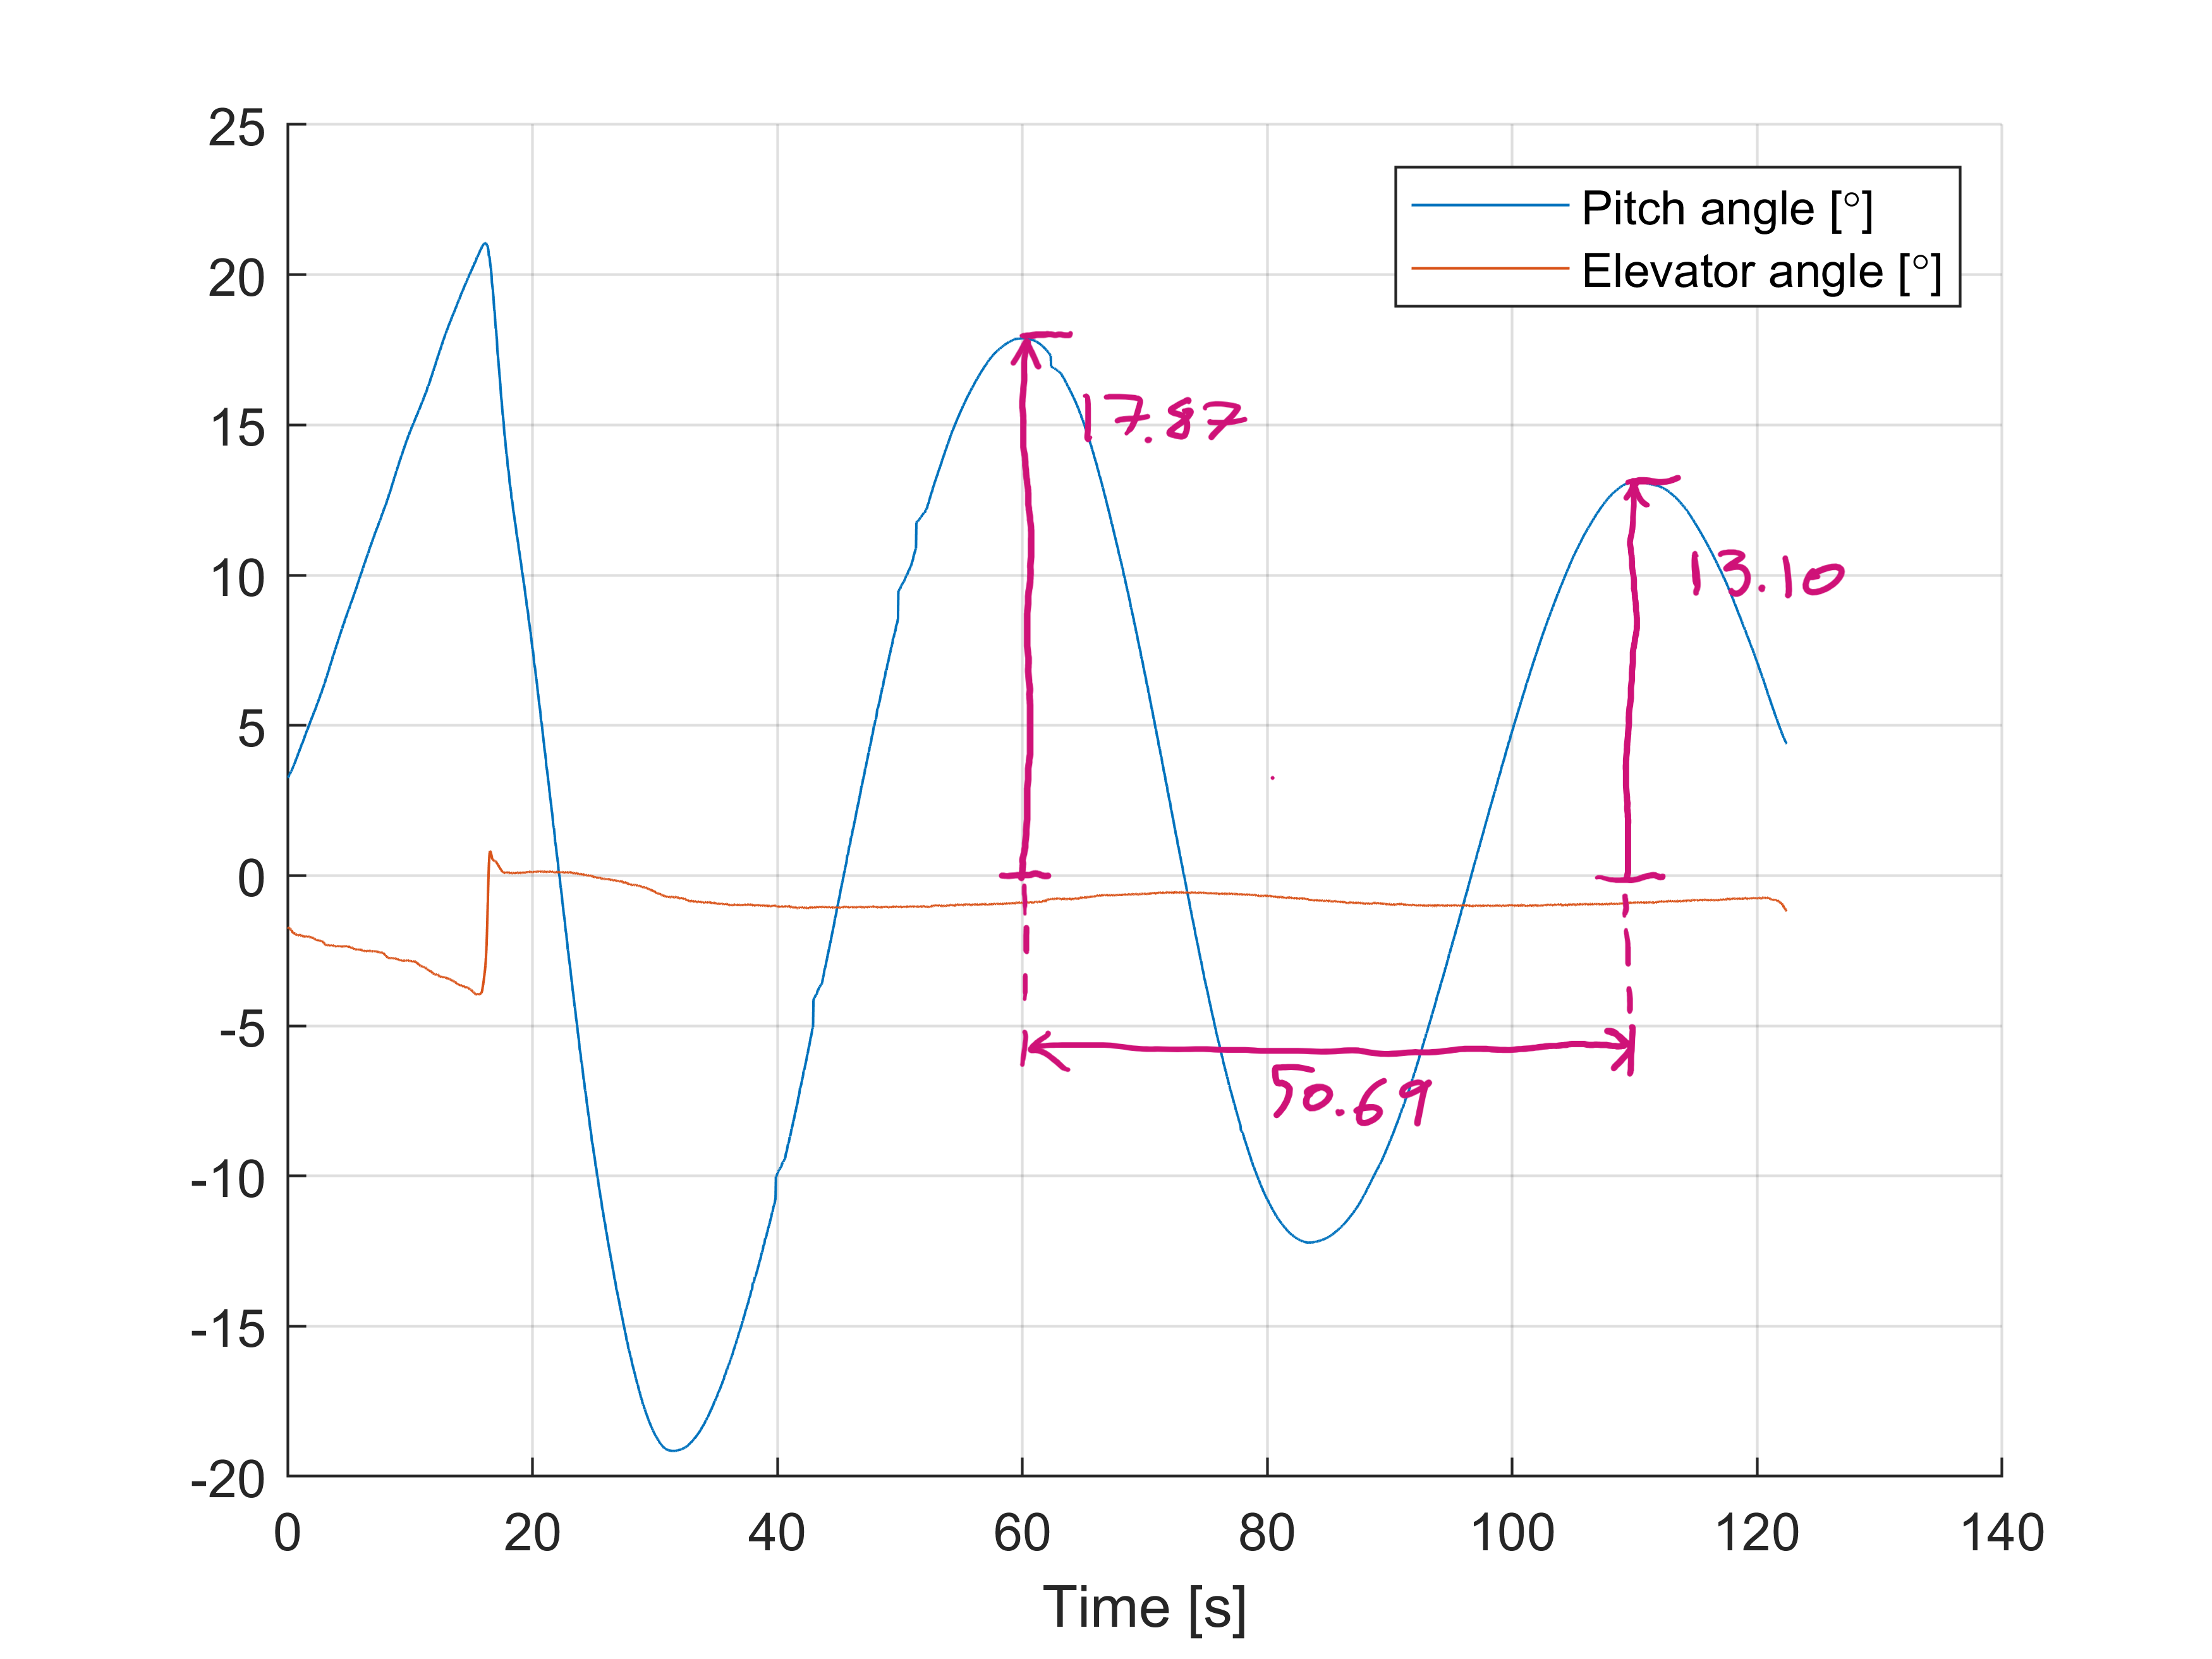
\includegraphics[width=0.8\textwidth]{figures/anPhugoid.png}
  \caption{}
  \label{fig:phugoid}
\end{figure}

\begin{figure}[H]
  \centering
  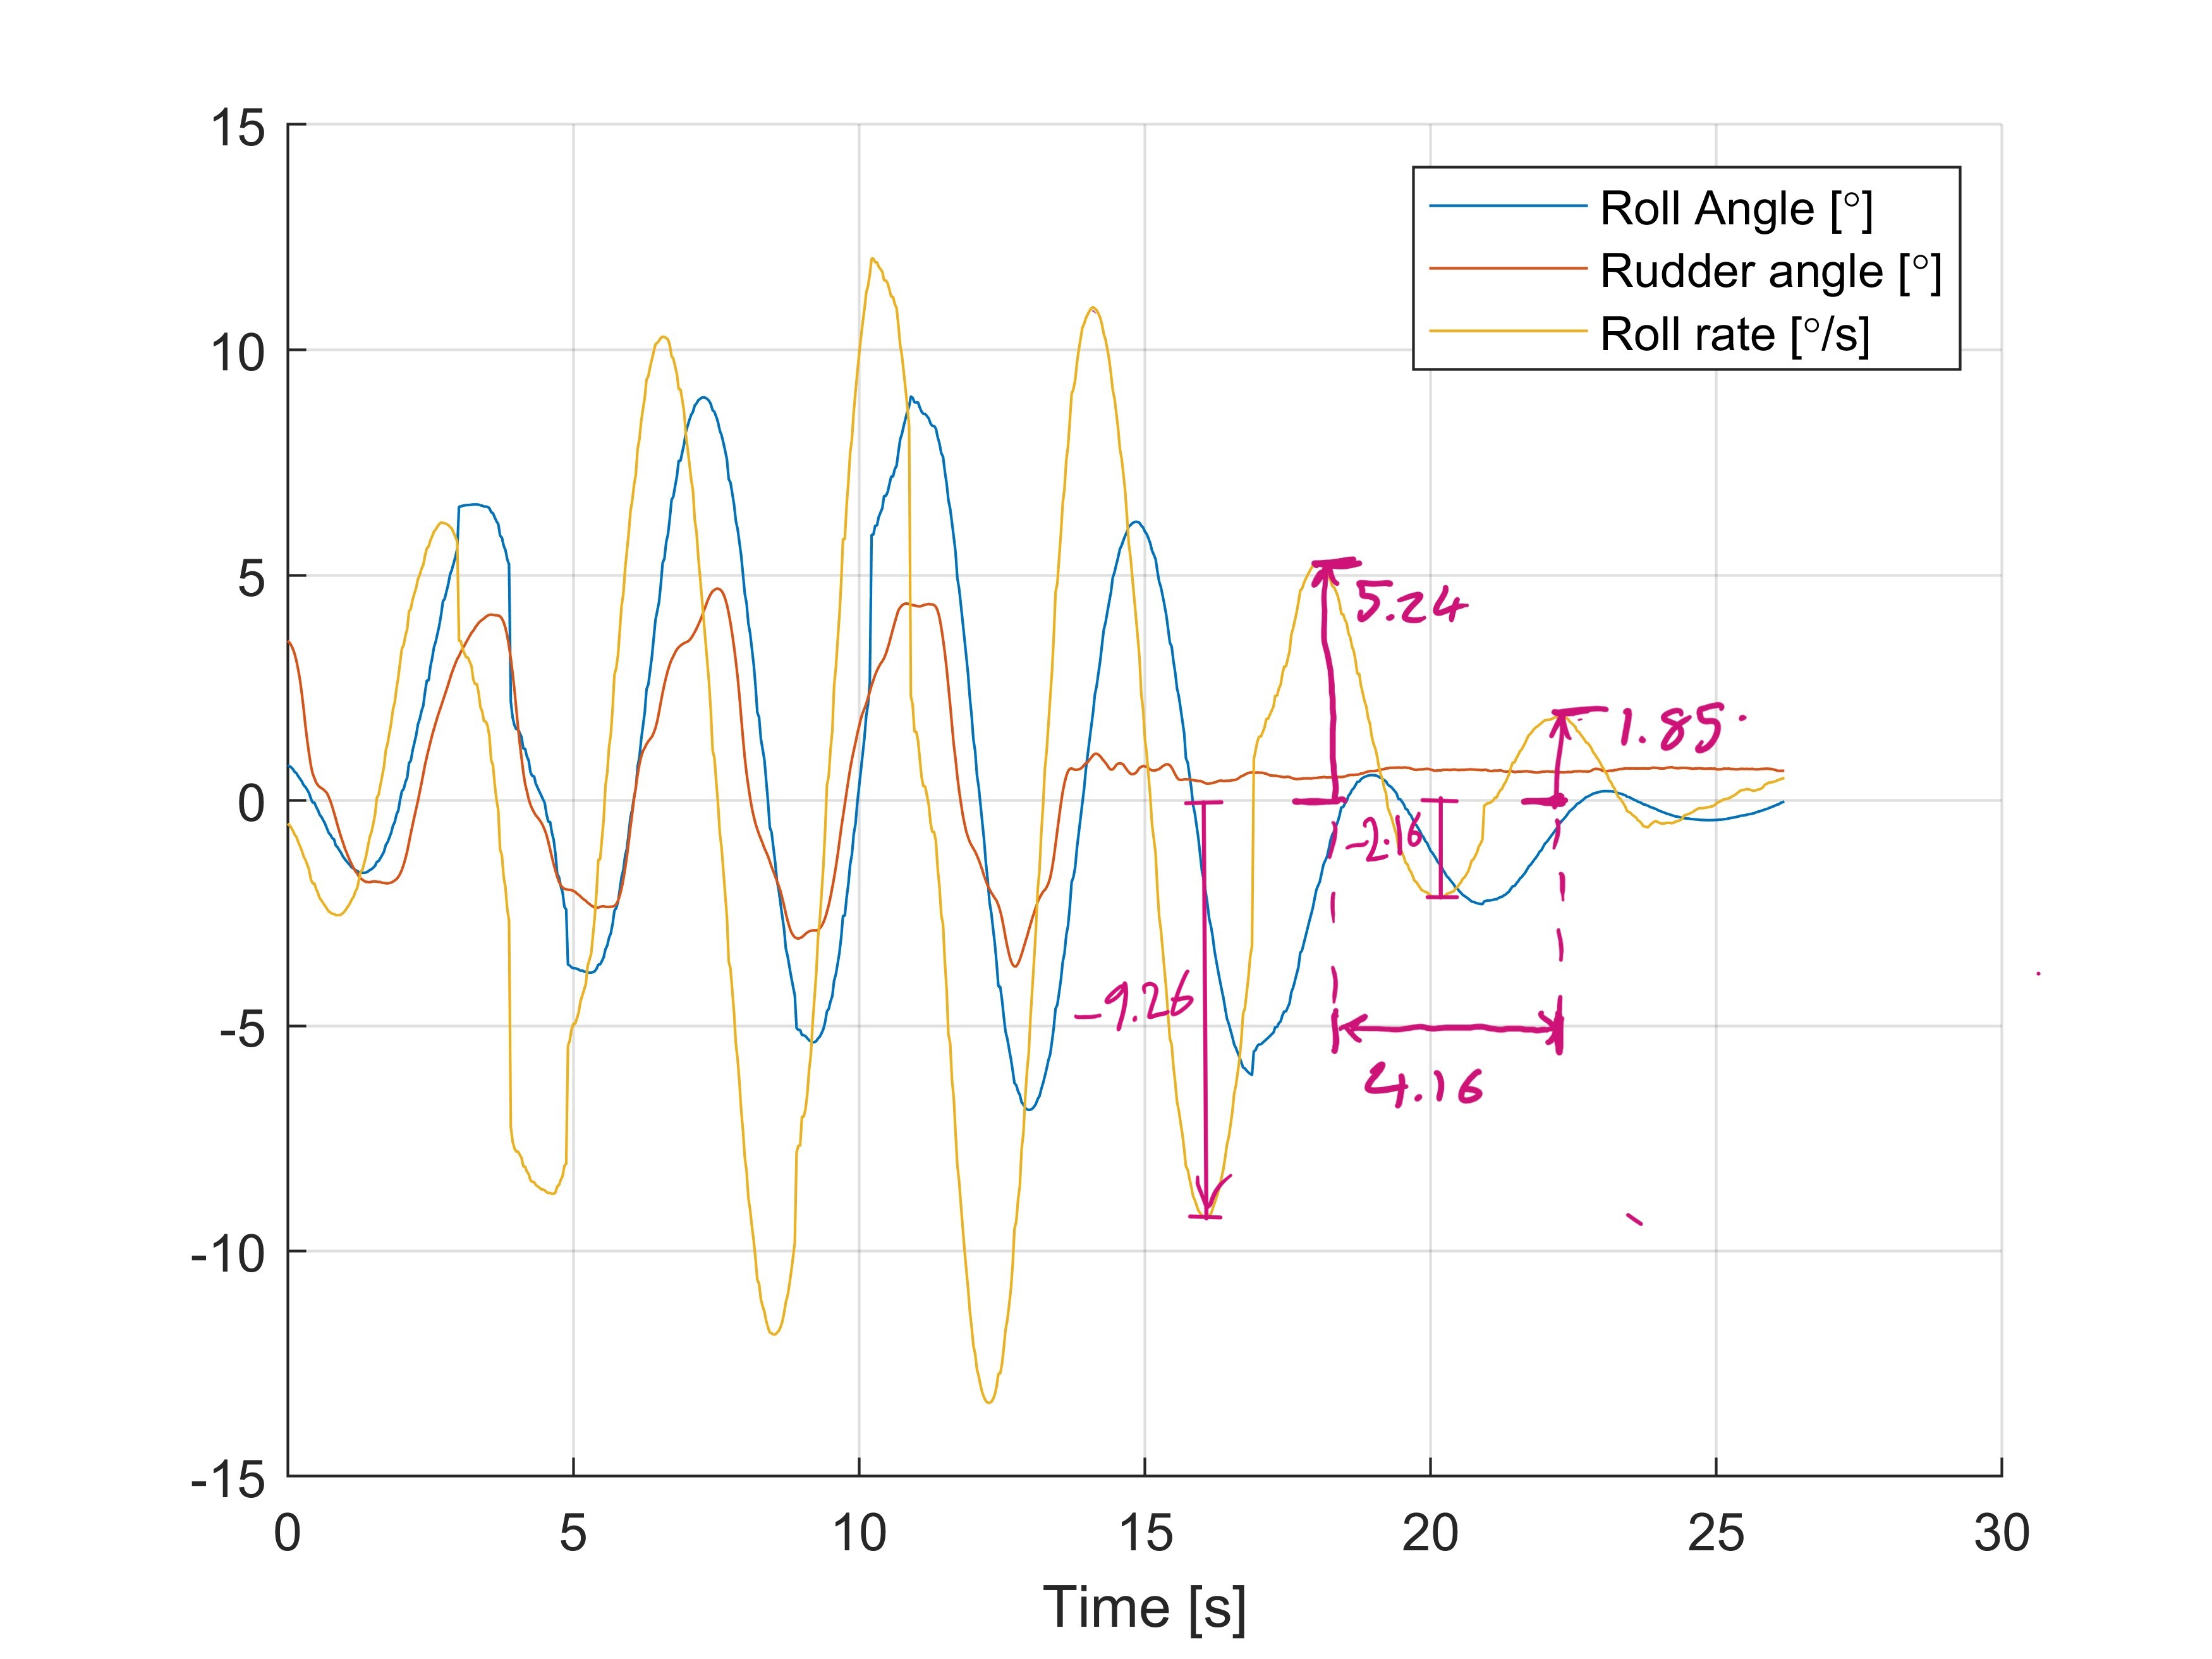
\includegraphics[width=0.8\textwidth]{figures/anDutchRoll.jpg}
  \caption{}
  \label{fig:dutchroll}
\end{figure}

\begin{figure}[H]
  \centering
  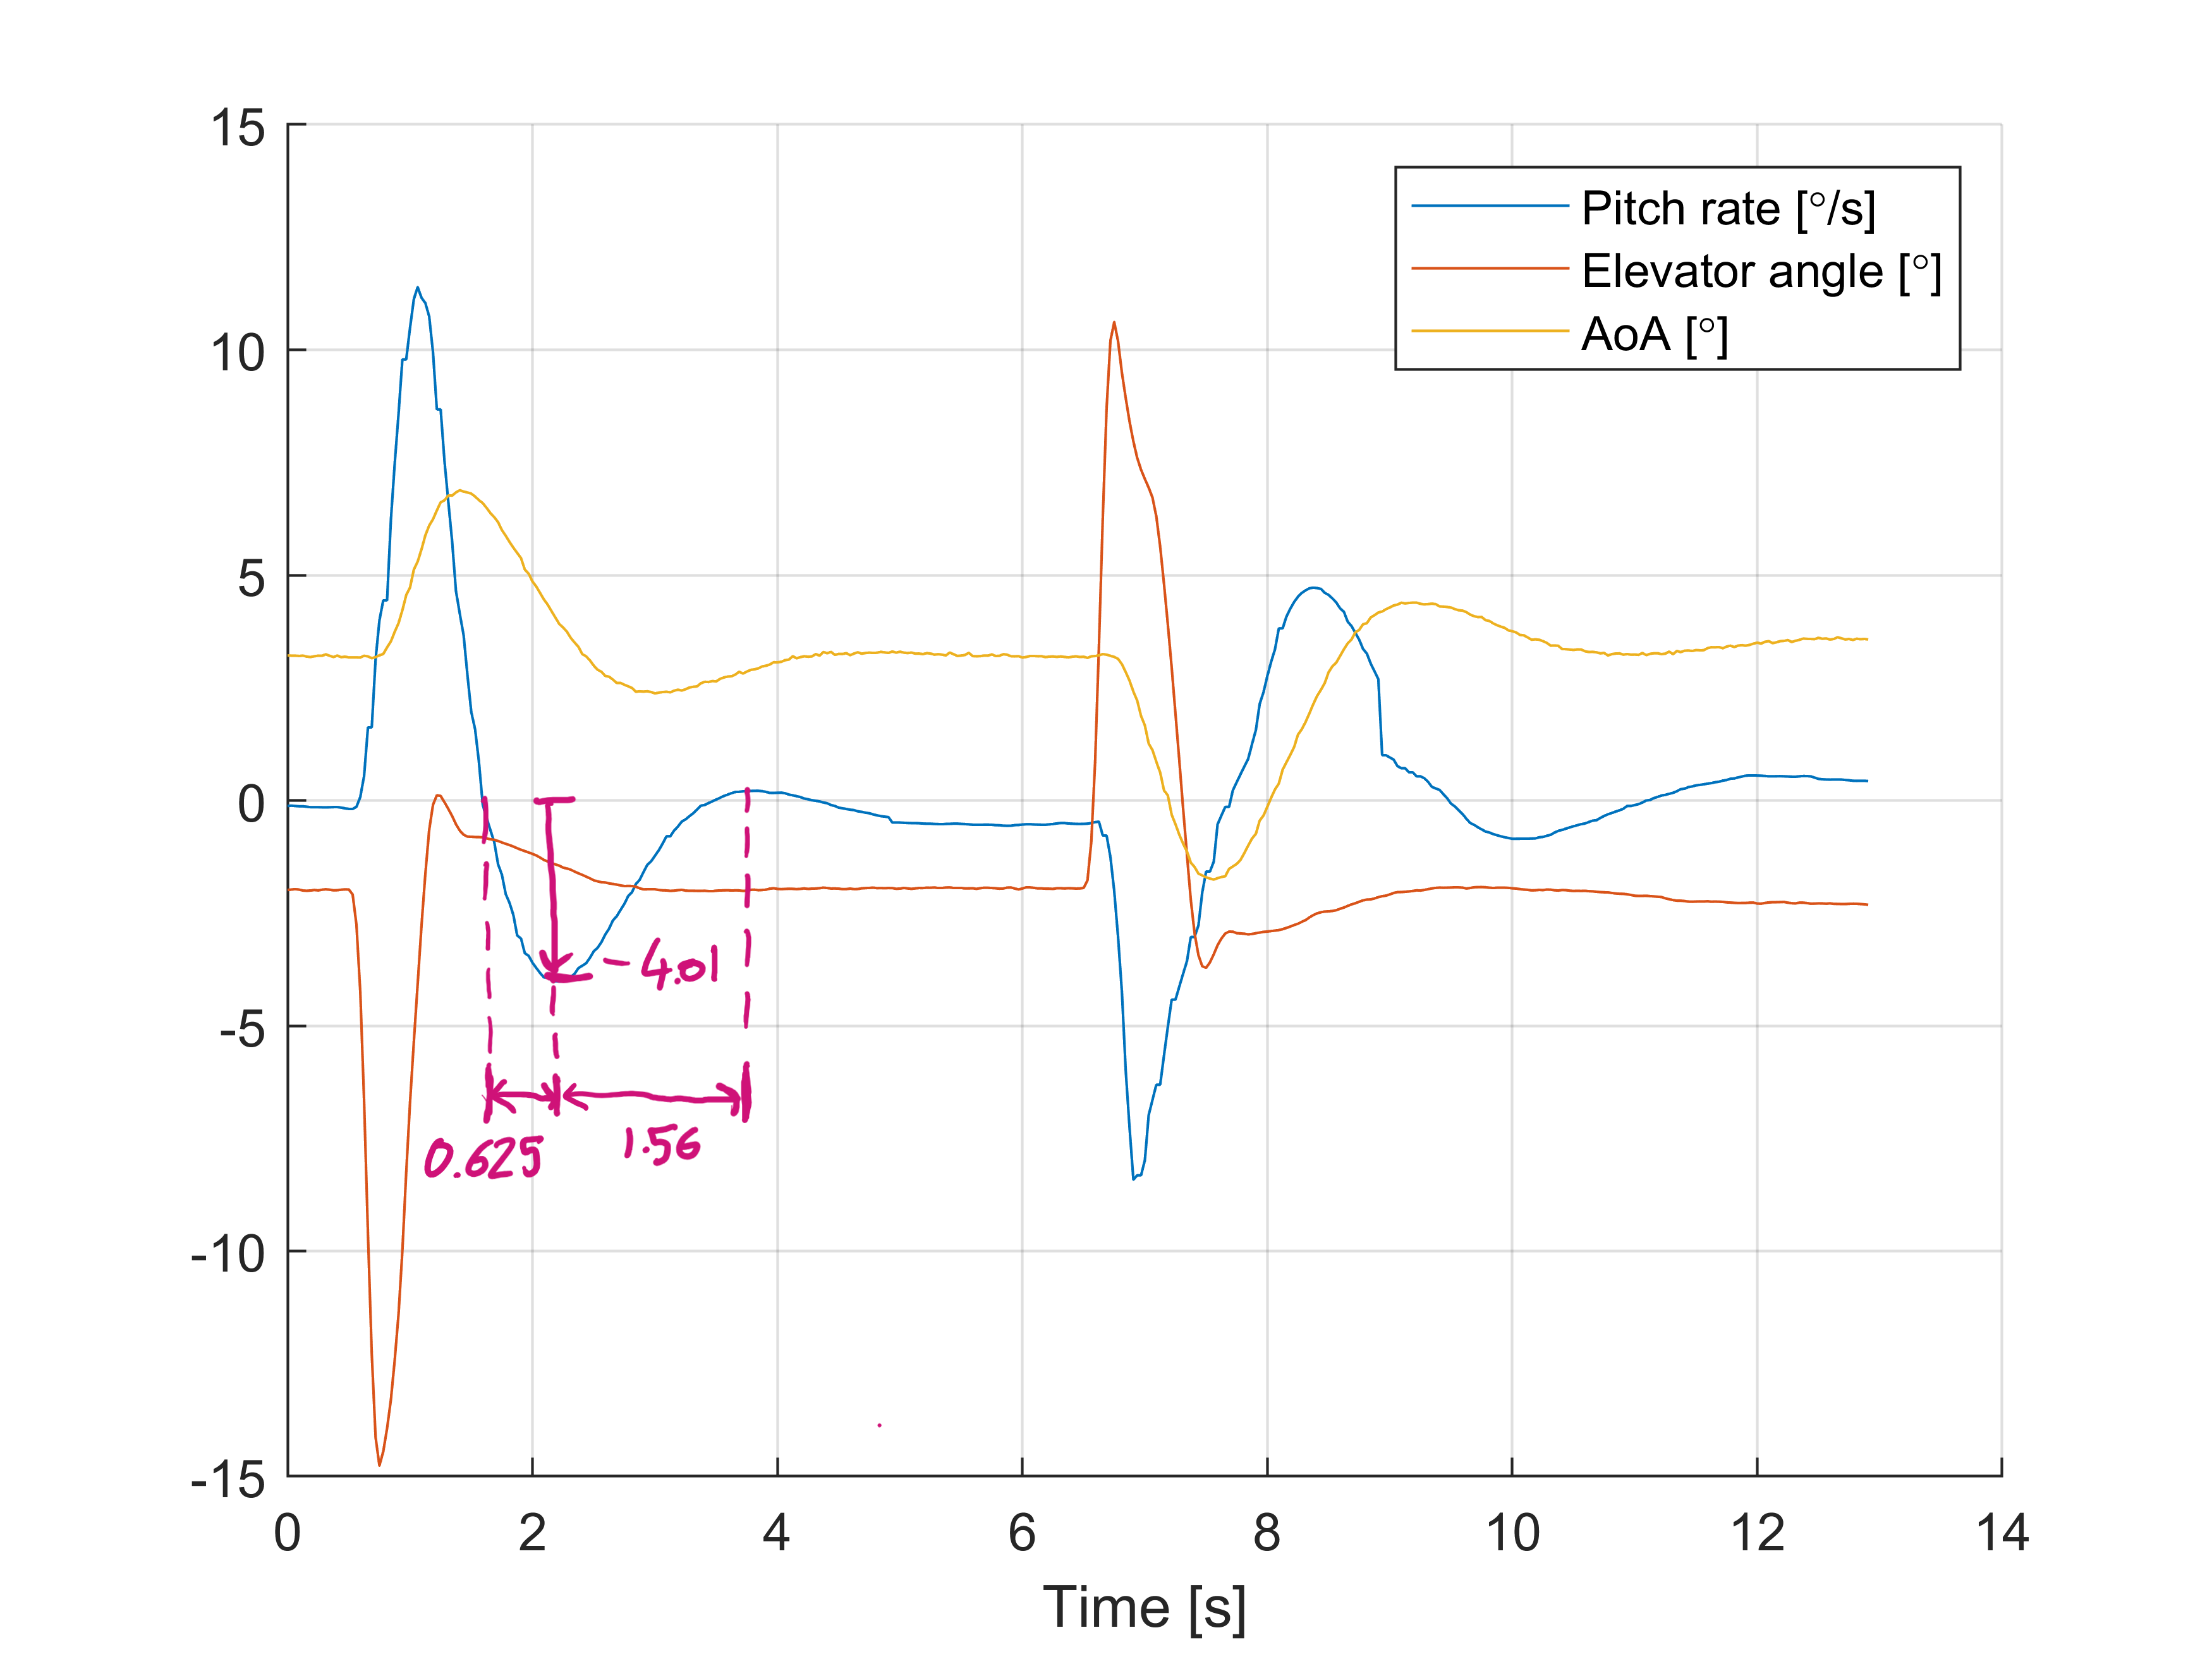
\includegraphics[width=0.8\textwidth]{figures/anSPO.png}
  \caption{}
  \label{fig:spo}
\end{figure}

This short period oscillation is highly damped and so is harder to obtain accurate modal characteristics.
The unforced part of the response, shown anotated in figure \ref{fig:spo} is matched to a decaying sine-wave shown in equation \ref{eq:spoeq}.
\begin{equation}
  y = Ae^{-\zeta\omega_{n}(t - t_{0})}\sin(\omega_{d}(t - t_{0})) + B
\end{equation}
Where
\begin{equation}
  \omega_{d} = \omega_{n}\sqrt{1 - \zeta^{2}}
\end{equation}
From the graph $t_0 = 1.625$, $B=-0.54$ and $\omega_d = 2\pi/1.56 = 4.03$.
The damping ratio is then a function of the phase of the first peak, $\psi_m = 0.56\omega_d$.
\begin{equation}
  \tan(\psi_m) = \frac{\sqrt(1-\zeta^2)}{\zeta}
\end{equation}
Rearranging and taking positive root gives $\zeta= 0.77$.
Then using the amplitude $y(t=t_0 + 0.56) = -3.47$ we can solve for $A$.


\begin{figure}[H]
  \centering
  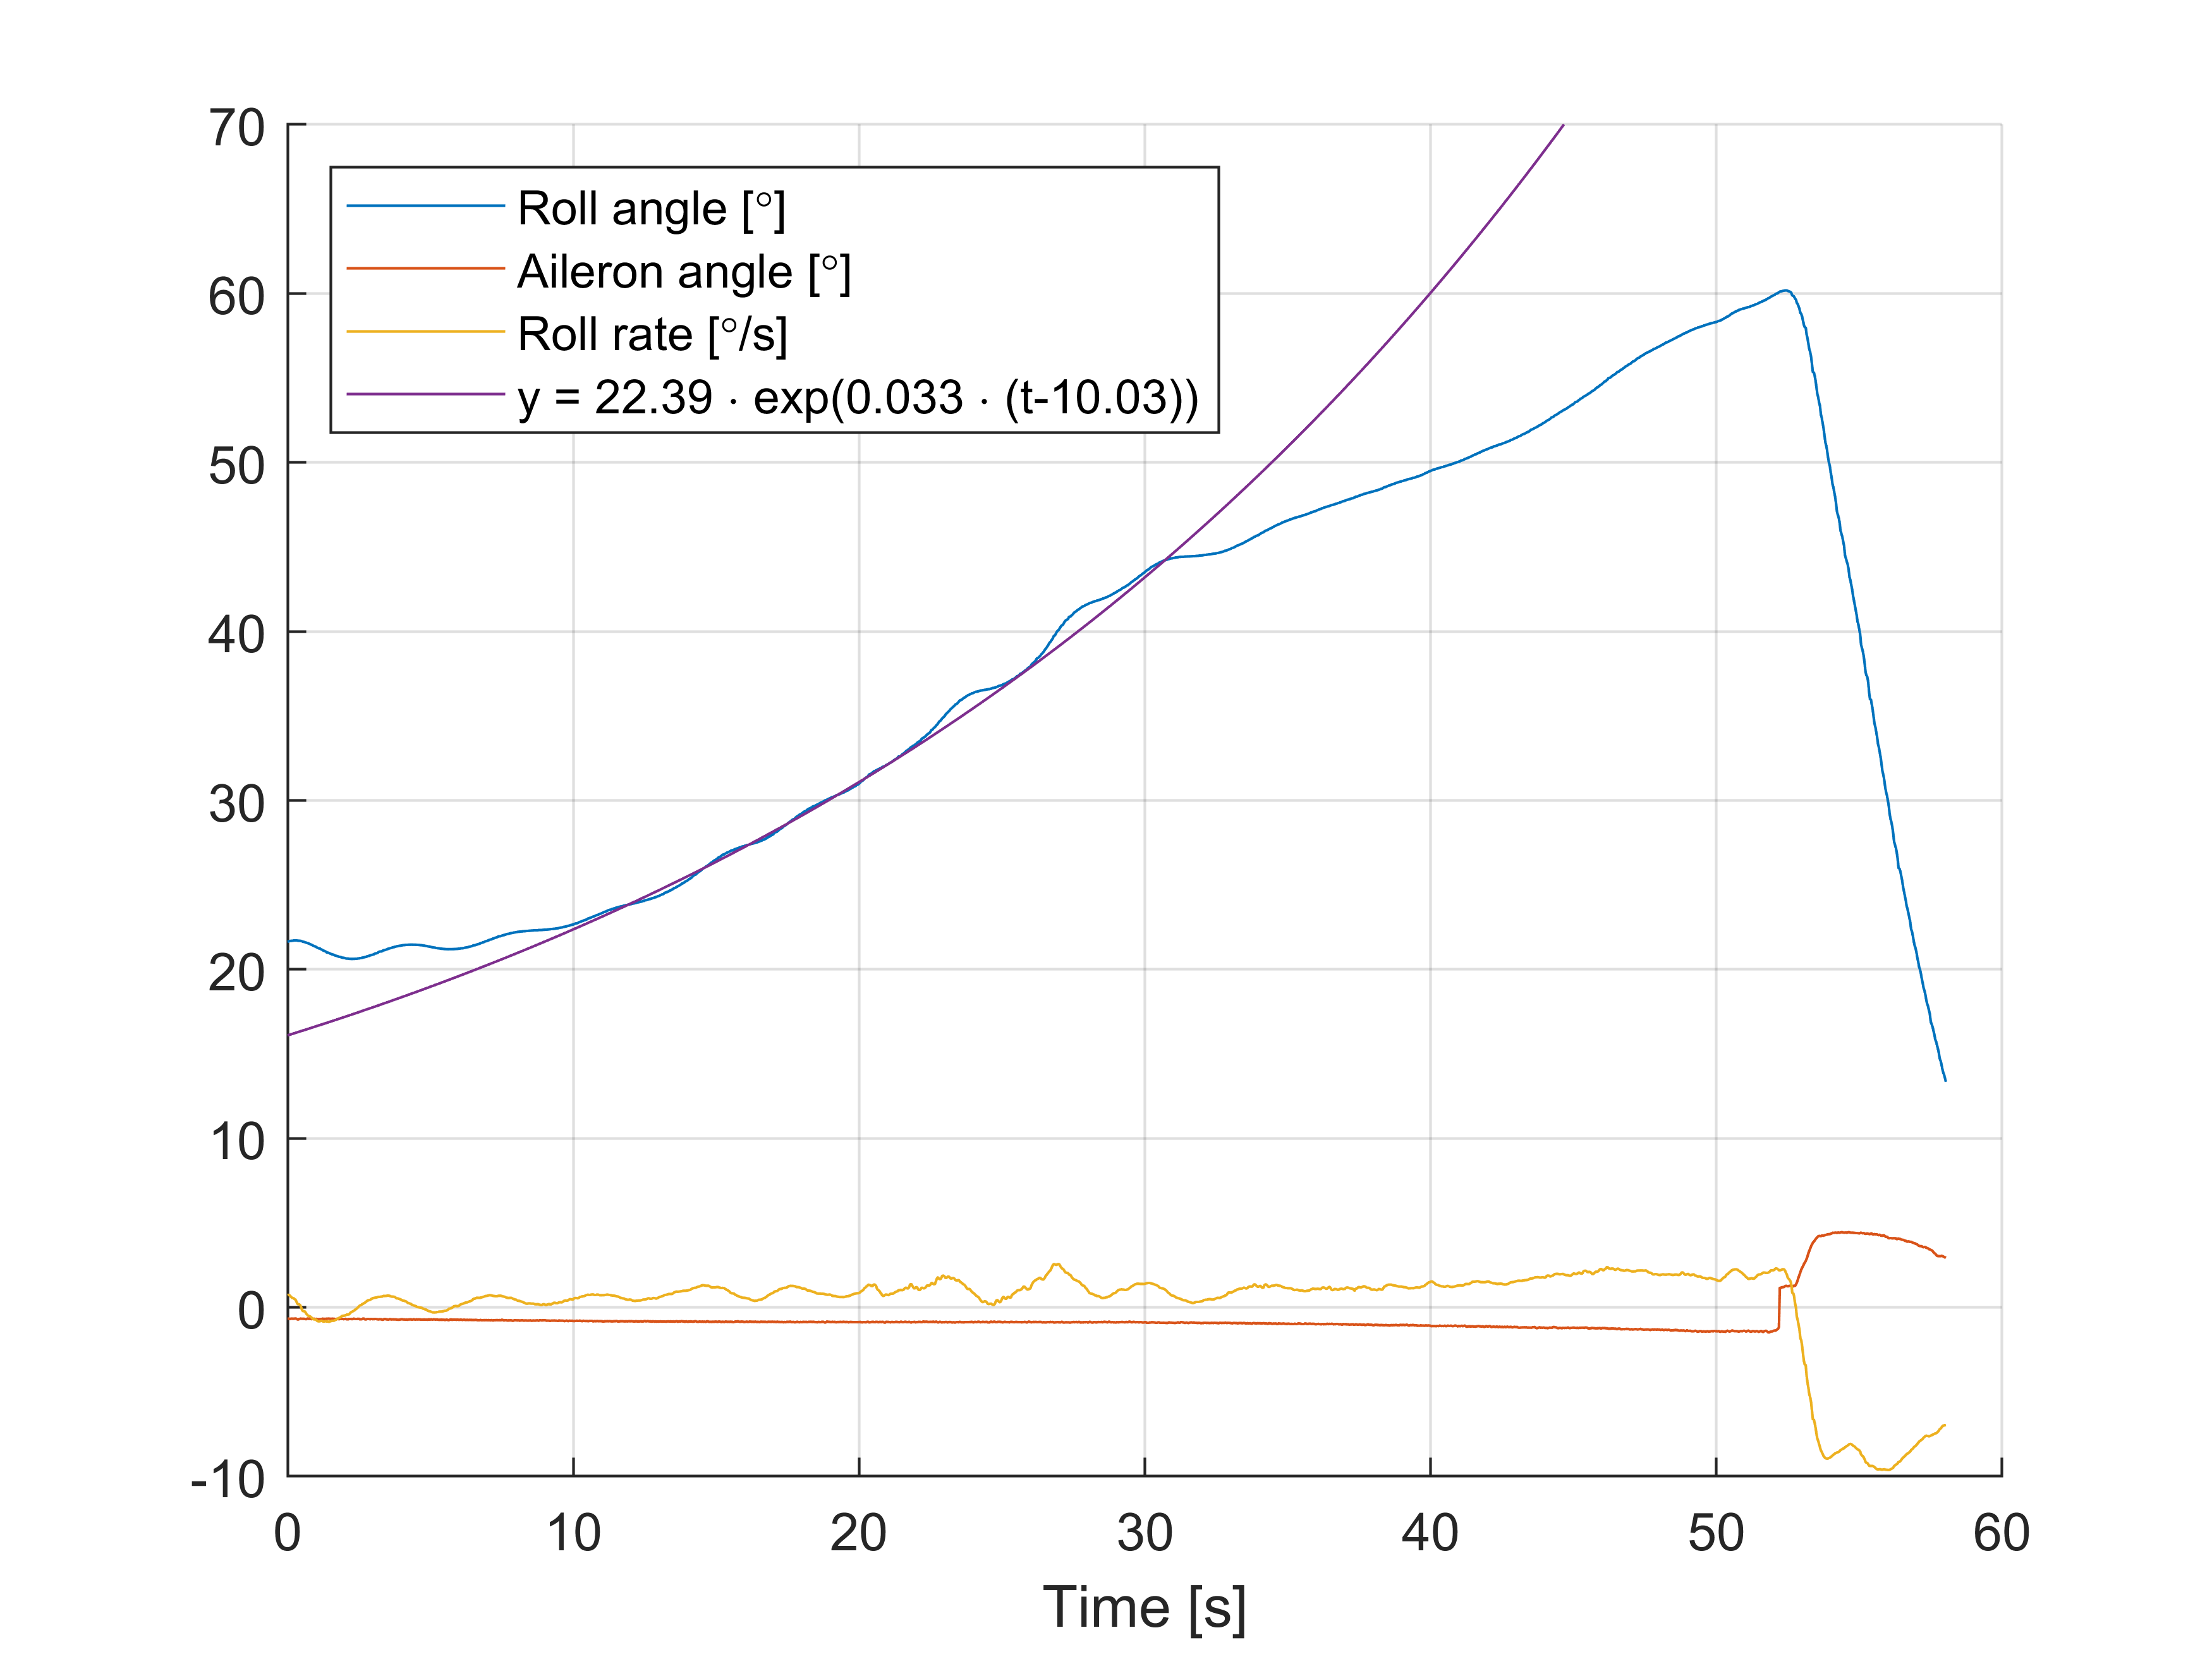
\includegraphics[width=0.8\textwidth]{figures/Spiral.png}
  \caption{}
  \label{fig:spiral}
\end{figure}

The region of interest was chosen for its little control input and small deviations from equilibrium to stay within linear theory.

\begin{figure}[H]
  \centering
  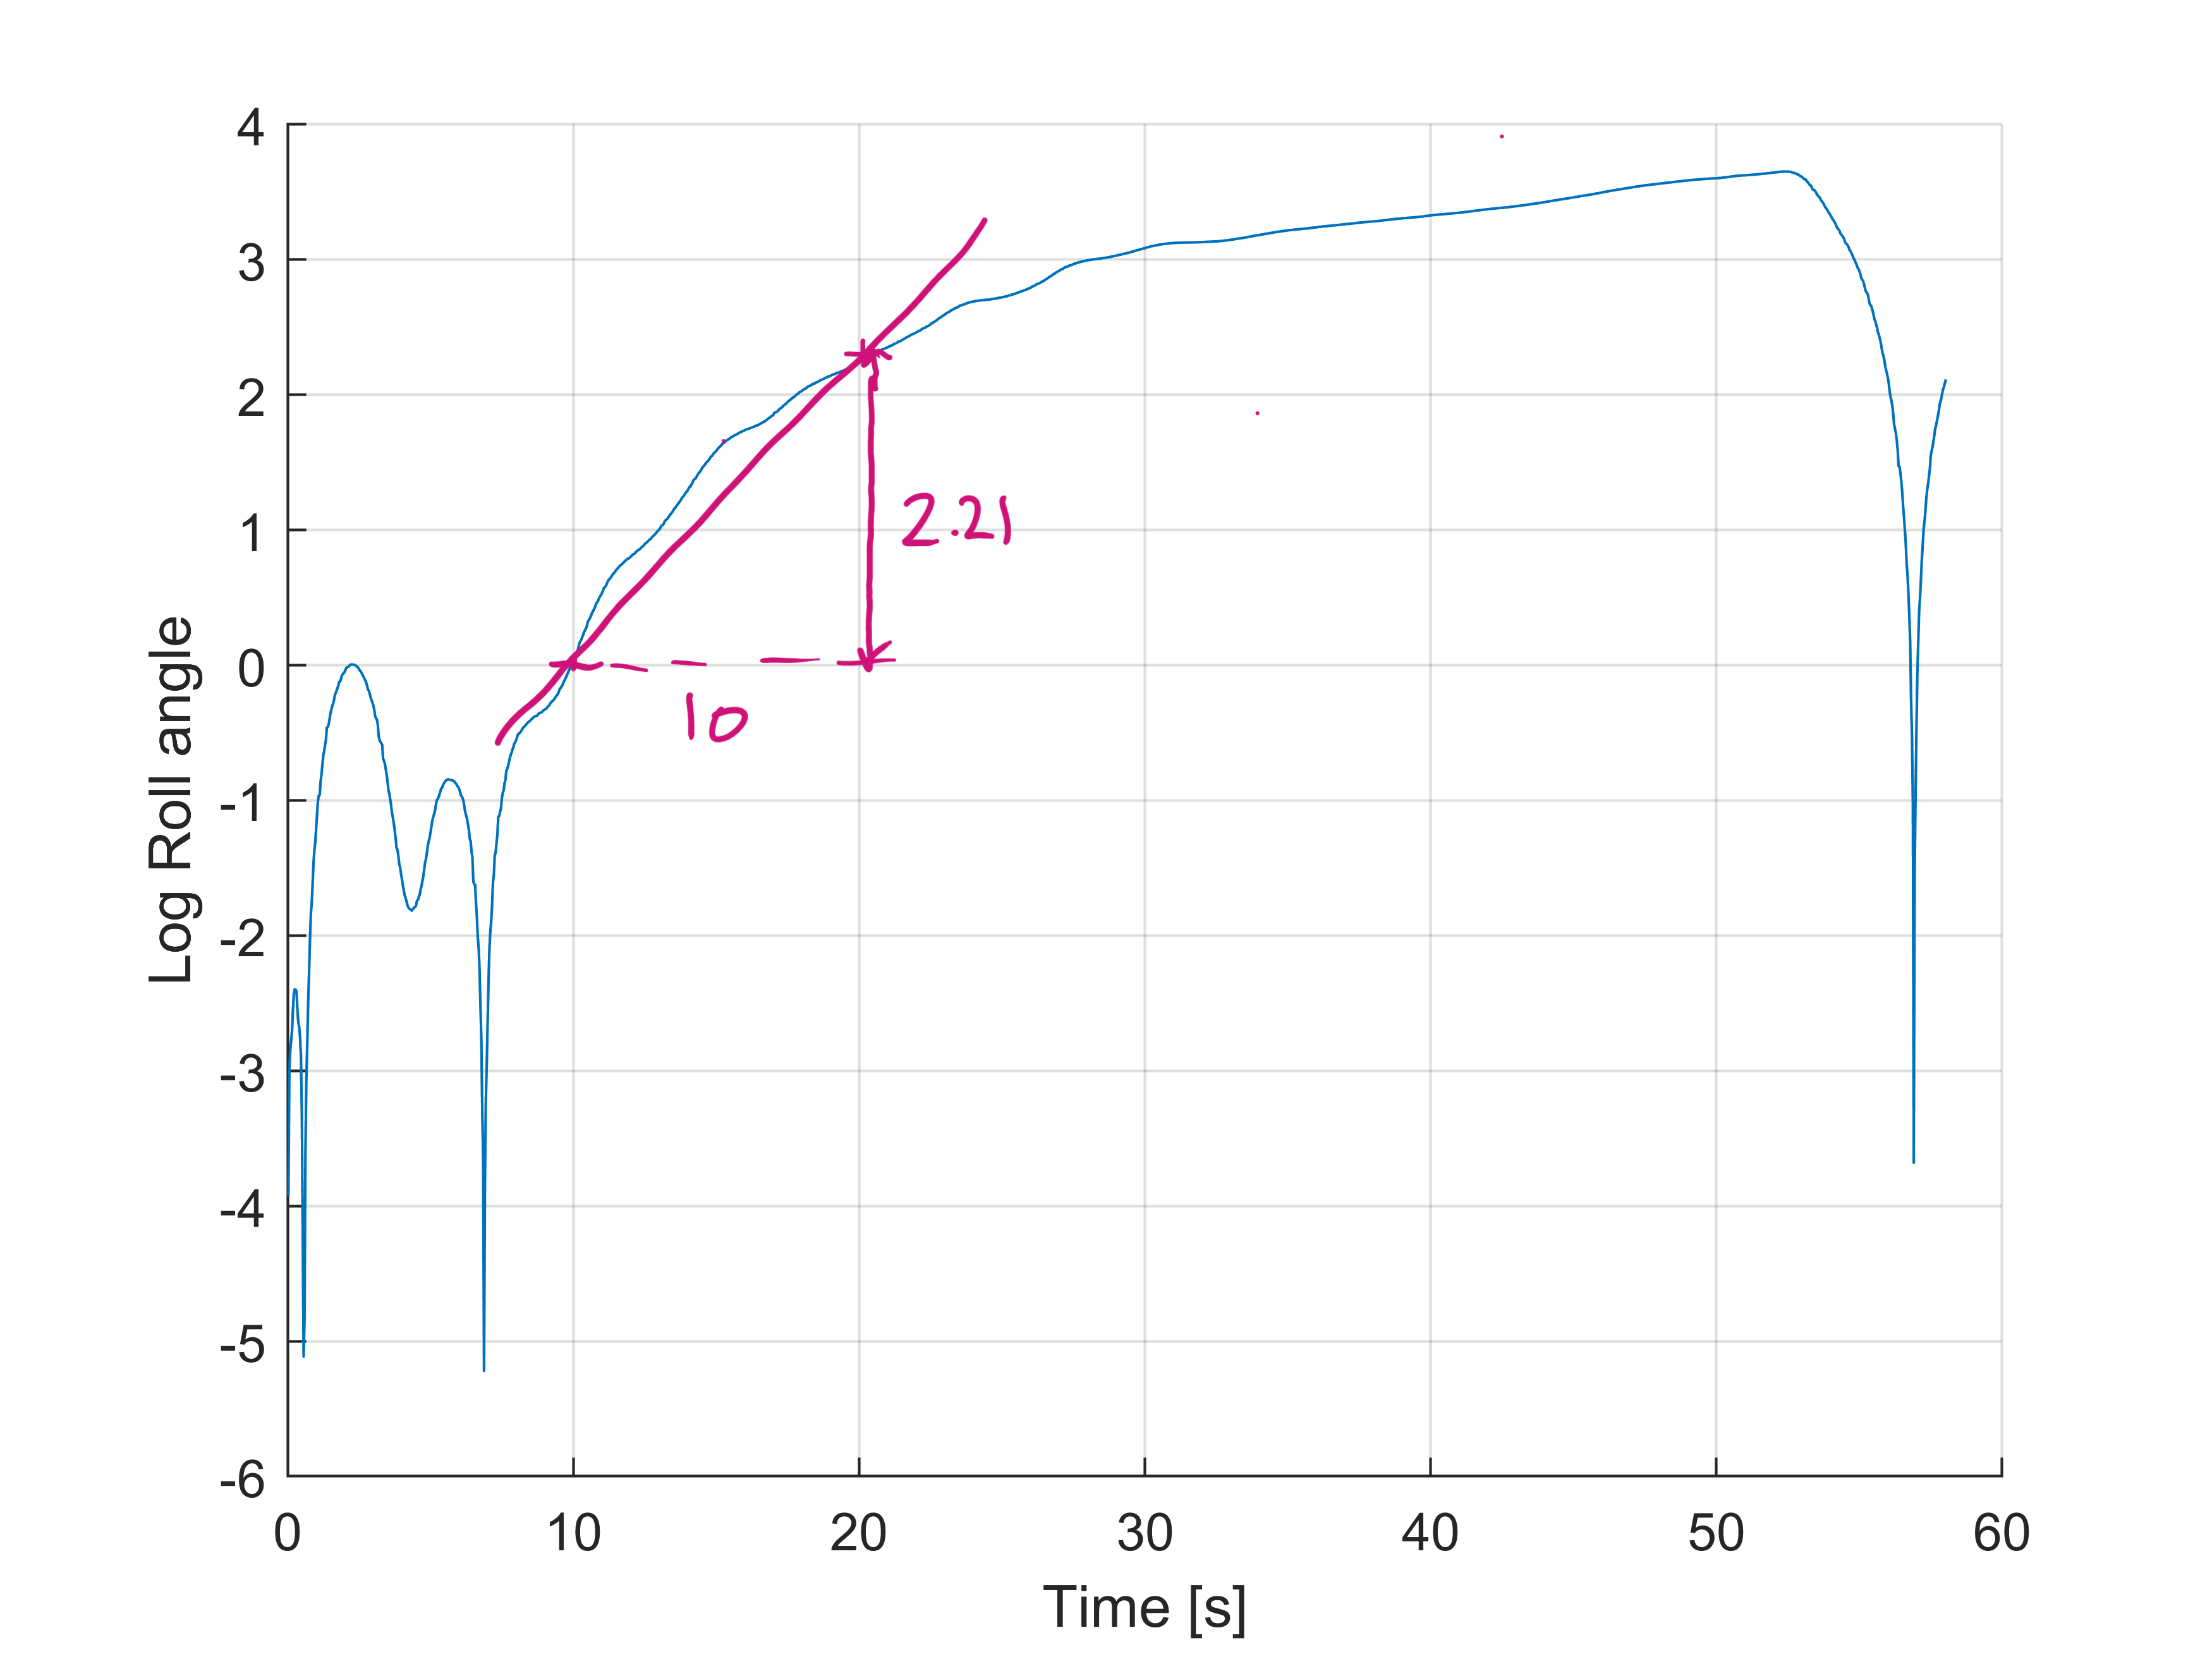
\includegraphics[width=0.8\textwidth]{figures/anSpiral_log.png}
  \caption{}
  \label{fig:spiral_log}
\end{figure}

Manual curve fitting was attempted by plotting $\log(\texttt{Rollang} - \texttt{Rollang}(1))$ against $\texttt{Time}$ to obtain the time constant,
This however was difficult because...


\begin{thebibliography}{9}

  \bibitem{handout}
  S. Place, A. Cooke
  \emph{Flight Experimental Methods: Course Handbook}
  Cranfield University,

\end{thebibliography}

\end{document}

